%!TEX root = ./main.tex

\section[Signal strength]{Attempt 1: Signal Strength}

% SECTION TIMING: 8:00--16:00 (2 frames). The obvious idea, given its fair chance,
% then killed by its own curve. Students must SEE why the ruler is too coarse
% before they will accept a stranger ruler (phase).

% Teaching note (150 s): left: power falls as 1/d^2, so a power reading is a
% distance. Right: three APs, three circles, one intersection -- trilateration,
% exactly what GPS does with time. This is how every phone OS started.
\begin{frame}{Attempt 1: louder means closer}
  \vspace{0.2em}
  \begin{columns}[T,onlytextwidth]
    \column{0.47\textwidth}
      \centering
      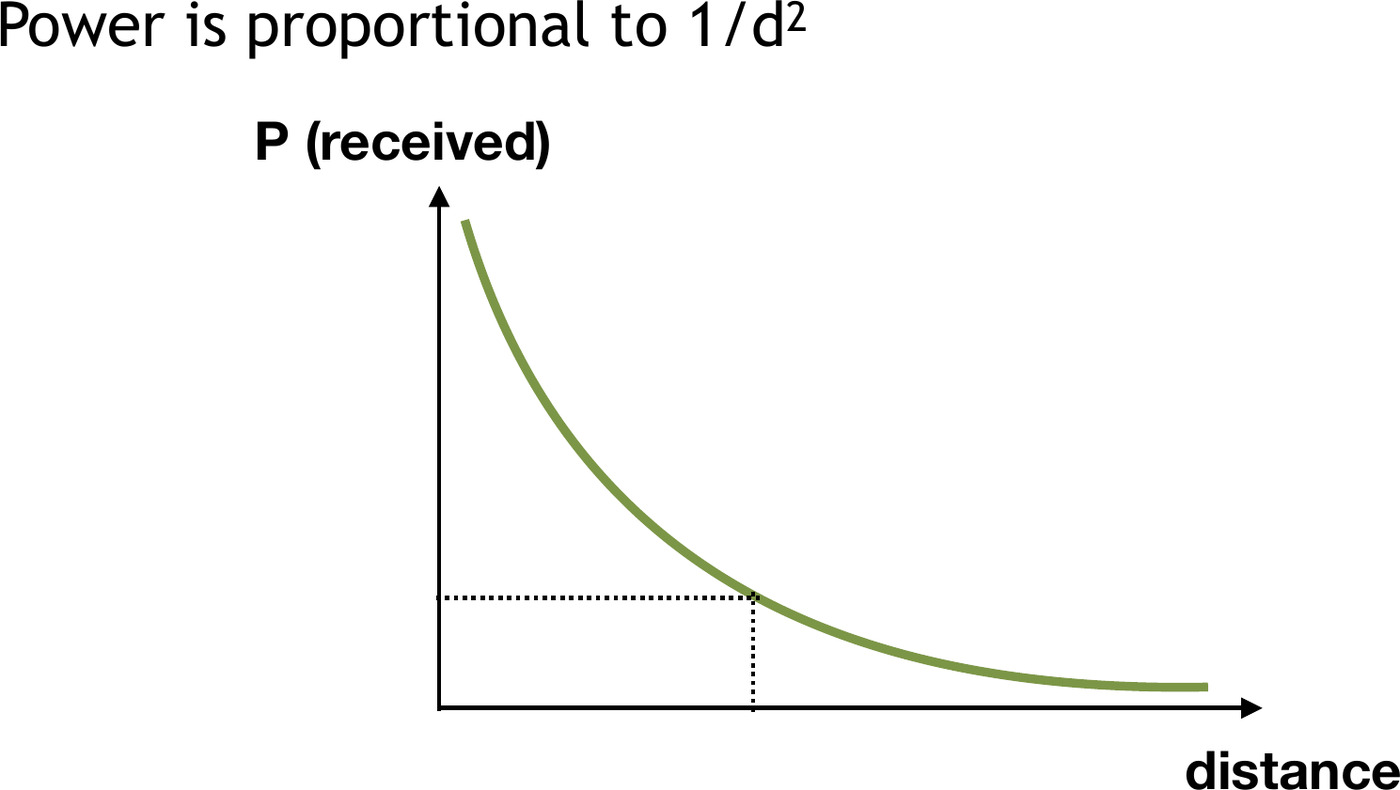
\includegraphics[width=\linewidth]{figure/mit_rssi_curve.png}
      {\small Power $\propto 1/d^2$: read a power, get a distance.\par}
    \column{0.49\textwidth}
      \centering
      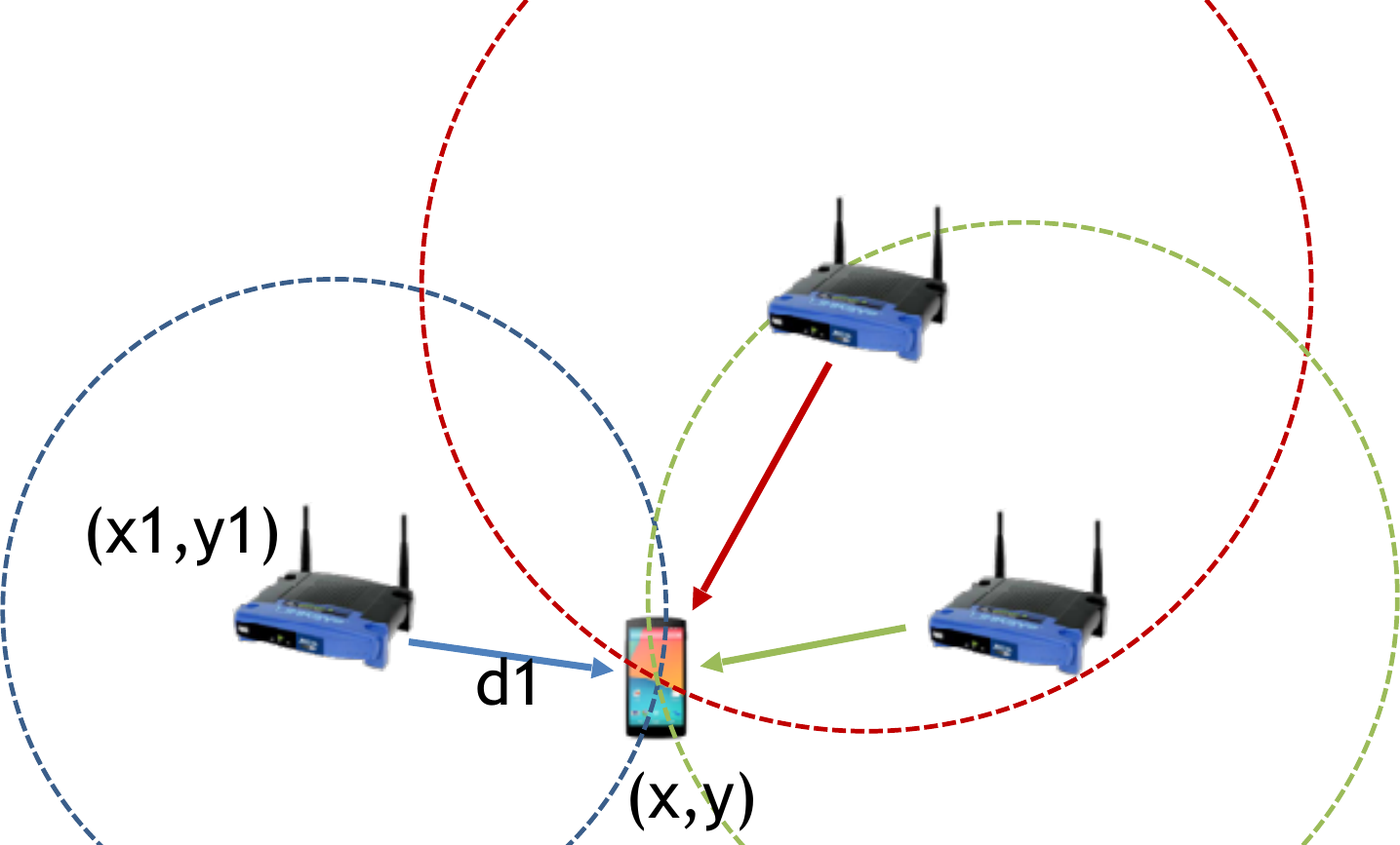
\includegraphics[width=\linewidth]{figure/mit_trilateration.png}
      {\small One distance per AP; the circles meet at the phone.\par}
  \end{columns}
  \source{https://www.mit.edu/~fadel/courses/MAS.s60/materials/Lec2-localization-2022.pdf}{Figures: MIT MAS.S60 Lecture 2}
\end{frame}

% Teaching note (180 s): two cons on the left curve -- far away the curve is flat
% (a small power error is a large distance error), and reflections make power wiggle
% with position. Right: the industry workaround -- walk the building and record a
% fingerprint at every orange dot. Works; room-level; must be redone when furniture
% moves. Verdict box, then move on.
\begin{frame}{Why RSSI stops at room level}
  \vspace{0.2em}
  \begin{columns}[T,onlytextwidth]
    \column{0.52\textwidth}
      \centering
      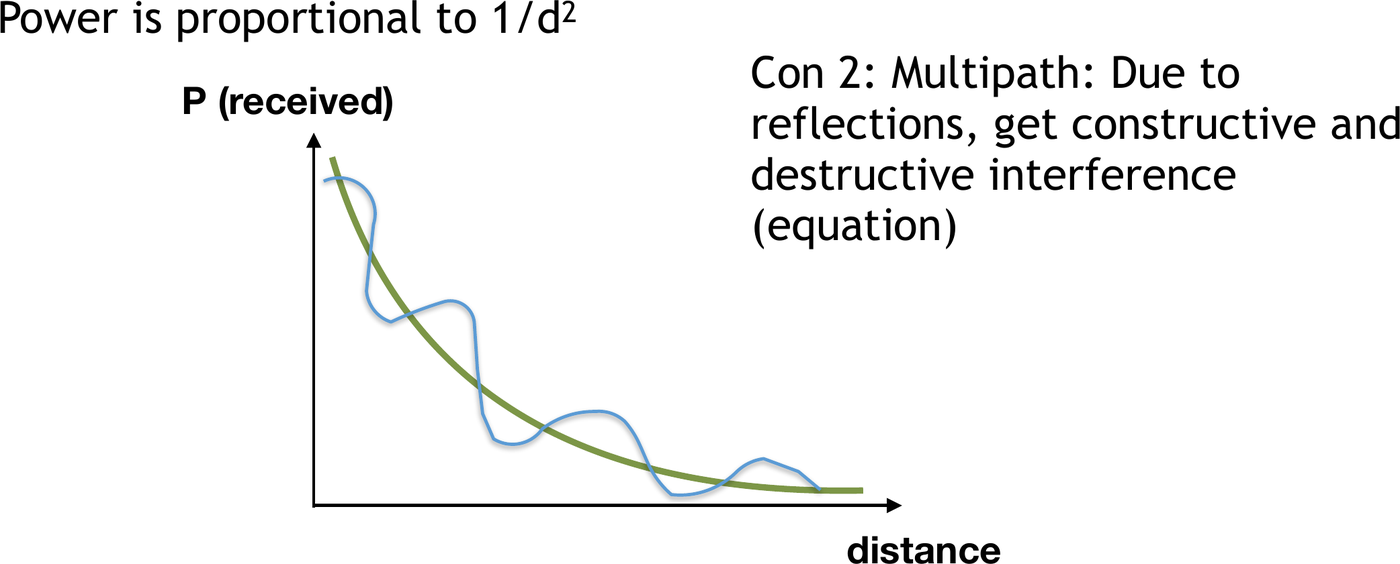
\includegraphics[width=\linewidth]{figure/mit_rssi_multipath.png}
      {\small Reflections add and cancel: power wiggles with position.\par}
    \column{0.44\textwidth}
      \centering
      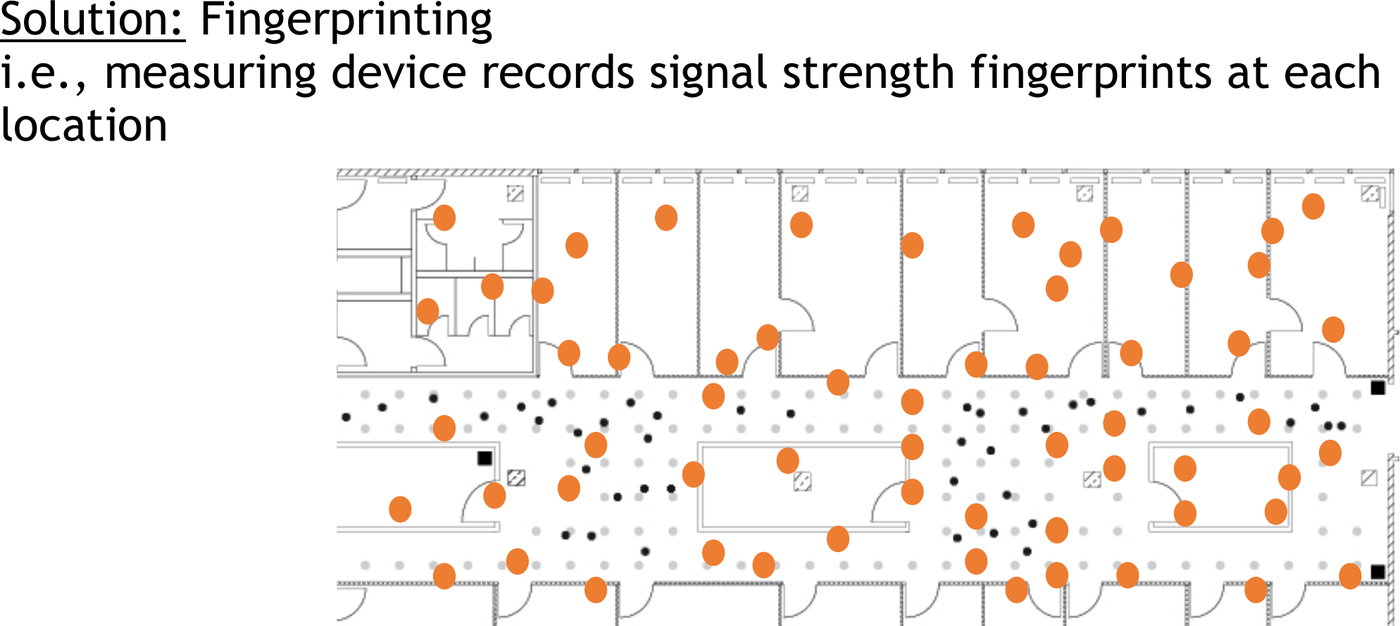
\includegraphics[width=\linewidth]{figure/mit_fingerprint.png}
      {\small Workaround: record a fingerprint at every dot.\par}
  \end{columns}

  \vspace{0.4em}
  \takeaway{One number per packet, summed over every reflection: \textbf{room-level}.\\
    For a desk-level answer we need a finer ruler.}
  \source{https://www.mit.edu/~fadel/courses/MAS.s60/materials/Lec2-localization-2022.pdf}{Figures: MIT MAS.S60 Lecture 2}
\end{frame}
